\section{Method}
\label{sec:method}

VolTilt uses two rules to construct the allocation in Section~\ref{sec:problem}. An LLM reads financial news and produces event records from which we derive the relative shares $q_{i,t}$. A volatility-targeting rule converts historical portfolio returns into the invested fraction $\lambda_t$ (Fig.~\ref{fig:overview}). We express the relative shares using the rank multiplier $\tau_{i,t}$ so that the capital weight is $a_{i,t}=\lambda_t q_{i,t}=\lambda_t\tau_{i,t}/N_t$. The exposure multiplier recorded by the backtest is $w_{i,t}=N_t a_{i,t}$. A backbone can be substituted through the event-record schema while the allocation rules remain fixed. Past news can still influence the invested fraction through the historical tilts used to estimate volatility.

\begin{figure}[tb]
\centering
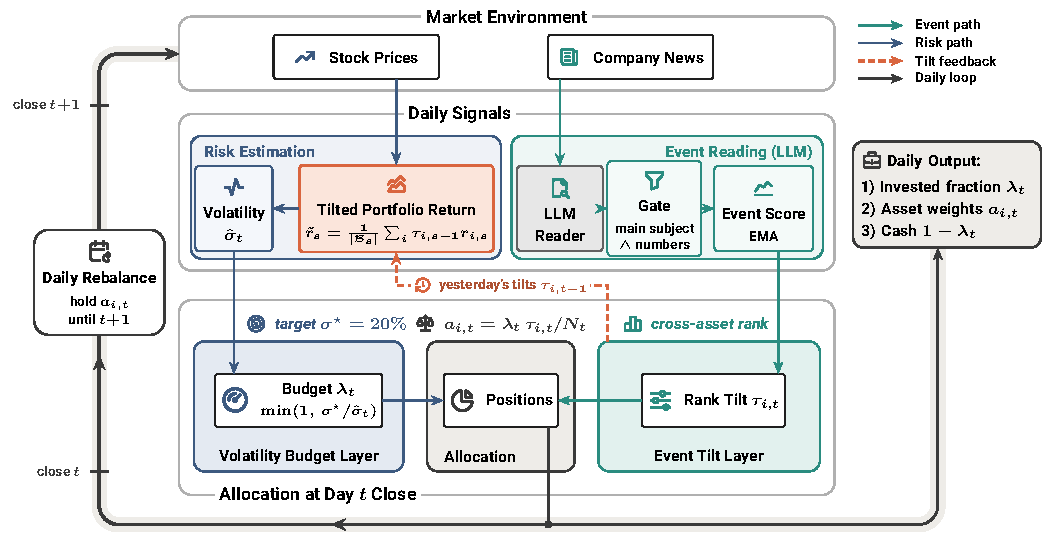
\includegraphics[width=\textwidth]{voltilt_arch.pdf}
\caption{VolTilt allocation at close $t$. The event path ranks smoothed news scores to set relative weights. The risk path scales invested capital using recent volatility. The dashed connection shows how past tilts enter the risk estimate through realised returns. We hold positions until the next rebalance.}
\label{fig:overview}
\end{figure}

\subsection{Structured Event Scoring}

For each asset--article pair, the LLM receives the company name and the first $1{,}500$ characters of the cleaned article. At temperature zero, it produces a record with five fields: \texttt{focus}, \texttt{event\_type}, \texttt{novelty}, \texttt{hard\_numbers}, and \texttt{impact}. The first identifies whether the company is the main subject, is mentioned in passing, or is unrelated. The next two identify one of twelve event categories and distinguish a new fact, follow-up, recap, or opinion. The Boolean \texttt{hard\_numbers} field indicates the presence of company-specific figures. We denote the signed impact by $u_i(x)\in\{-2,-1,0,1,2\}$. The prompt asks for a judgement of the effect of new information over the following week, with zero representing neutral or already-priced information. The prompt instructs the model to use the article alone and judge the impact of new information. The categories cover earnings, guidance, analyst actions, products, legal events, deals, management, supply or demand, aggregate conditions, price recaps, opinions, and other reports. We cache records by the SHA-256 hash of the dataset asset identifier and original article text. Only successfully parsed records enter the score. Articles with missing cache entries contribute nothing.

Let $\mathcal{G}_{i,t}\subseteq\mathcal{X}_{i,t}$ contain the reports that identify the company as the main subject and contain company-specific figures. The gate restricts the signal to company-specific quantitative disclosures. Event type and novelty are retained as metadata. We assess the gate against a main-subject-only control. We sum the impact judgements for the qualifying articles and smooth the daily scores:
$h_{i,t}=\sum_{x\in\mathcal{G}_{i,t}}u_i(x)$ and $s_{i,t}=(1-\alpha)s_{i,t-1}+\alpha h_{i,t}$~\ieq{eq:vt-score}.
We update the EMA once per panel date, including warm-up and dates without qualifying articles, using $s_{i,0}=0$ and $\alpha=2/21$. When $h_{i,t}=0$, the previous score decays. Summation treats increments on the ordinal scale as additive and can give repeated coverage more weight. We compare it with a count-based signal and with averaging the qualifying scores (Section~\ref{sec:experiments}).

\subsection{Bounded Cross-Asset Tilt}

Building on the use of news scores in portfolio weighting~\cite{anic2025systematic}, we use the ordering of the smoothed scores in Eq.~\eqref{eq:vt-score}. The model supplies ordinal impact judgements, and the rank transformation requires no calibration of the scores as expected returns. Let $\rho_{i,t}$ be the ascending rank of $s_{i,t}$ among the $N_t$ assets in $\mathcal{A}_t$, with average ranks for ties. For a universe of at least three assets and at least two eligible assets on day $t$, we set
$\tau_{i,t}=1+k\,\bigl(\rho_{i,t}-(N_t+1)/2\bigr)/\bigl((N_t-1)/2\bigr)$ with $k=0.5$~\ieq{eq:vt-rank}.
We use unit tilts when all scores tie, fewer than two assets are eligible, or the chosen universe contains at most two assets. Ranks discard differences in score magnitude. Small differences can therefore produce different weights, and two distinct scores in a pair would force the full tilt spread. The tilt-off rule for two-asset universes was selected on a design sample. Section~\ref{sec:experiments} describes that selection and tests sensitivity to the fixed tilt strength $k$.

The ranks sum to $N_t(N_t+1)/2$, so the tilts average one and each lies in $[1-k,1+k]$. Thus $q_{i,t}=\tau_{i,t}/N_t$ is nonnegative and sums to one. The resulting risky capital weights sum to $\lambda_t$ and each lies in $[0,1]$. At a fixed budget, the fraction of capital transferred relative to equal shares is bounded by
\begin{equation}
  \frac{1}{2}\sum_{i\in\mathcal{A}_t}\left|a_{i,t}-\frac{\lambda_t}{N_t}\right|
  =\frac{\lambda_t}{2N_t}\sum_{i\in\mathcal{A}_t}|\tau_{i,t}-1|
  \leq\frac{k\lambda_t}{2}.
  \label{eq:vt-transfer}
\end{equation}
The factor of one half counts each reallocation once. The bound applies to weight changes induced by the rank rule at a given invested fraction. The matched-budget comparison tests their effect on realised performance.

\subsection{Volatility-Conditioned Exposure}

VolTilt estimates risk from the historical return series of the unscaled allocations, following work on volatility-managed strategies~\cite{barroso2015moments,moreira2017volmanaged}. For each panel date $s\le t$, let $\mathcal{B}_s$ contain the assets with a price return ending at $s$. The implementation computes $r^{\mathrm{obs}}_{i,s}=p_{i,s}/p_{i,s_i^-}-1$ between the asset's consecutive observed closes, with $s_i^-$ as defined in Section~\ref{sec:problem}. It multiplies each return by the tilt from the preceding panel date and takes the mean across the observed legs:
$\tilde r_s=\frac{1}{|\mathcal{B}_s|}\sum_{i\in\mathcal{B}_s}\tau_{i,s-1}\,r^{\mathrm{obs}}_{i,s}$~\ieq{eq:vt-history}.
An observed-close return can span a gap in the price panel. We use a unit tilt when the asset has no tilt at the preceding panel date. If a return is missing, we omit that leg and divide by the number of observed legs, without rescaling the remaining tilts to sum to that number. A date with no observed return leaves a missing value in the volatility history. This convention can change effective weights when observations are missing. We construct the series before cash scaling and turnover costs so a prior cut in the invested fraction cannot lower the estimated volatility mechanically.

We compute $\hat\sigma_t$ from the trailing 20 panel dates of $\tilde r_s$, using a standard deviation with divisor 20 and annualisation by $\sqrt P$. With target $\sigma^\star=0.20$, we set
$\lambda_t=\min\bigl(1,\sigma^\star/\hat\sigma_t\bigr)$ and $a_{i,t}=\lambda_t\tau_{i,t}/N_t$~\ieq{eq:vt-budget}.
We use $\lambda_t=1$ when the rolling window does not contain 20 returns or the estimate is zero. When estimated volatility exceeds the target, the rule scales every risky weight proportionally and leaves $1-\lambda_t$ in cash. The target governs scaling based on historical volatility. Future realised volatility can exceed it.

Today's budget depends on earlier relative allocations. The dependency runs from the preceding tilts through realised returns to the budget, $\boldsymbol{\tau}_{s-1}\to\tilde r_s\to\hat\sigma_t\to\lambda_t$ for sessions $s$ in the rolling window. Today's news changes today's relative allocation immediately under the benchmark's timing convention. That tilt first enters the volatility estimate when a subsequent return is observed. Across backbones the sizing rule is fixed, while the sequence of daily budgets can vary.

\subsection{Controlled Allocation Variants}

The news-aware portfolio $(\lambda^{\mathrm{news}},q^{\mathrm{news}})$ uses the rank tilt throughout Eqs.~\eqref{eq:vt-history} and~\eqref{eq:vt-budget}. For the news-neutral portfolio $(\lambda^{\mathrm{eq}},q^{\mathrm{eq}})$, we set every tilt to one and recompute budget history with the same rule. Their Sharpe difference gives the policy contrast in Eq.~\eqref{eq:policy-contrast}, which includes any changes in invested fractions induced by historical tilts. For the matched-budget diagnostic, we apply the budget path $\lambda^{\mathrm{eq}}$ to both compositions. This gives the composition contrast in Eq.~\eqref{eq:composition-contrast}. We also swap the two budget paths while holding composition fixed to examine how historical tilts affect exposure. Section~\ref{sec:experiments} reports these contrasts alongside shifted-score, article-count, and one-session-delay checks. The matched-budget contrast fixes daily invested capital and leaves realised risk and trading costs free to differ. It describes the performance consequences of changing relative weights under that budget path. The full policy contrast also captures the change in the budget induced by past tilts. When the universe has at most two assets, unit tilts make the full and volatility-only policies identical under common inputs and accounting.
